\chapter{Qt Formen}
\begin{figure}[H]
	\begin{subfigure}{0.245\textwidth}
		\centering
		\begin{tikzpicture}[every node/.style={black, fill ,circle, inner sep = 1pt}]
		\node[label = {$V_0$}, rotate = 135] at (0,0) (V0) {};
		\node[label = {$V_1$}, rotate = -45] at (1,1) (V1) {};
		\node[label = {$V_2$}, rotate = 135] at (2,0) (V2) {};
		\node[label = {$V_3$}, rotate = -45] at (3,1) (V3) {};
		
		\draw (V0) -- (V1) (V2) -- (V3);
		\end{tikzpicture}
		\caption{\texttt{GL\_LINES}}
	\end{subfigure}
	%
	\begin{subfigure}{0.245\textwidth}
			\centering
		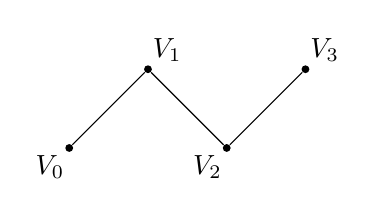
\begin{tikzpicture}[every node/.style={black, fill ,circle, inner sep = 1pt}]
		\node[label = {$V_0$}, rotate = 135] at (0,0) (V0) {};
		\node[label = {$V_1$}, rotate = -45] at (1,1) (V1) {};
		\node[label = {$V_2$}, rotate = 135] at (2,0) (V2) {};
		\node[label = {$V_3$}, rotate = -45] at (3,1) (V3) {};
		
		\draw (V0) -- (V1) -- (V2) -- (V3);
		\end{tikzpicture}
		\caption{\texttt{GL\_LINE\_STRIP}}
	\end{subfigure}
	%
	\begin{subfigure}{0.245\textwidth}
				\centering
		\begin{tikzpicture}[every node/.style={black, fill ,circle, inner sep = 1pt}]
		\node[label = {$V_0$}, rotate = 135] at (0,0) (V0) {};
		\node[label = {$V_1$}, rotate = -45] at (1,1) (V1) {};
		\node[label = {$V_2$}, rotate = 135] at (2,0) (V2) {};
		\node[label = {$V_3$}, rotate = -45] at (3,1) (V3) {};
		\end{tikzpicture}
		\caption{\texttt{GL\_POINTS}}
	\end{subfigure}
	%
	\begin{subfigure}{0.245\textwidth}
				\centering
		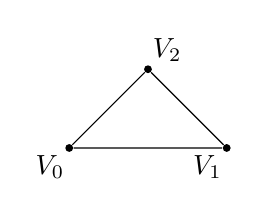
\begin{tikzpicture}[every node/.style={black, fill ,circle, inner sep = 1pt}]
		\node[label = {$V_0$}, rotate = 135] at (0,0) (V0) {};
		\node[label = {$V_2$}, rotate = -45] at (1,1) (V2) {};
		\node[label = {$V_1$}, rotate = 135] at (2,0) (V1) {};
		\draw (1,.4) node[fill=none, align=center, anchor=center] {\leftturn};
		\draw (V0) -- (V1) -- (V2) -- (V0);
		\end{tikzpicture}
		\caption{\texttt{GL\_TRIANGLE}}
	\end{subfigure}
	%
	\begin{subfigure}{.45\textwidth}
		\centering
		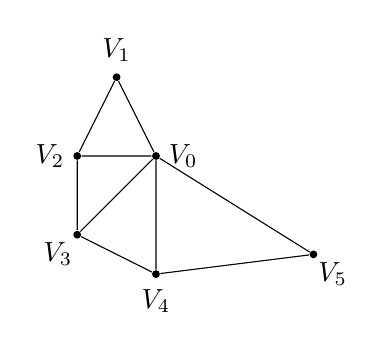
\begin{tikzpicture}[every node/.style={black, fill ,circle, inner sep = 1pt}]
			\node[label = {$V_0$}, rotate=-90] at (0,0) (V0) {};
			\node[label = {$V_1$}, rotate=0] at (-.5,1) (V1) {};
			\node[label = {$V_2$}, rotate=90] at (-1,0) (V2) {};
			\node[label = {$V_3$}, rotate=135] at (-1,-1) (V3) {};
			\node[label = {$V_4$}, rotate=180] at (0,-1.5) (V4) {};
			\node[label = {$V_5$}, rotate=-135] at (2,-1.25) (V5) {};
			
			\draw (V0) -- (V1) -- (V2)
			(V0) -- (V2) -- (V3)
			(V0) -- (V3) -- (V4)
			(V0) -- (V4) -- (V5) -- (V0);
		\end{tikzpicture}
		\caption{\texttt{GL\_TRIANGLE\_FAN}}
	\end{subfigure}
	%
	\begin{subfigure}{.45\textwidth}
			\centering
			\begin{tikzpicture}[every node/.style={black, fill ,circle, inner sep = 1pt}, xscale = 1.5]
			\node[label = {$V_0$}, rotate=180] at (0,0) (V0) {};
			\node[label = {$V_1$}, rotate=0] at (0,1) (V1) {};
			\node[label = {$V_2$}, rotate=180] at (1,0) (V2) {};
			\node[label = {$V_3$}, rotate=0] at (1,1) (V3) {};
			\node[label = {$V_4$}, rotate=180] at (2,0) (V4) {};
			\node[label = {$V_5$}, rotate=0] at (2,1) (V5) {};
			\node[label = {$V_6$}, rotate=180] at (3,0) (V6) {};
			\node[label = {$V_7$}, rotate=0] at (3,1) (V7) {};
			
			\draw (V0) -- (V1) -- (V2) -- (V0)
			(V1) -- (V2) -- (V3) -- (V1)
			(V2) -- (V3) -- (V4) -- (V2)
			(V3) -- (V4) -- (V5) -- (V3)
			(V4) -- (V5) -- (V6) -- (V4)
			(V5) -- (V6) -- (V7) -- (V5);
			
			\draw ($ 1/3*(V0)+1/3*(V1)+1/3*(V2)$) node[fill=none] {\rightturn};
			\draw ($ 1/3*(V1)+1/3*(V2)+1/3*(V3)$) node[fill=none] {\leftturn};
			\draw ($ 1/3*(V2)+1/3*(V3)+1/3*(V4)$) node[fill=none] {\rightturn};
			\draw ($ 1/3*(V3)+1/3*(V4)+1/3*(V5)$) node[fill=none] {\leftturn};
			\draw ($ 1/3*(V4)+1/3*(V5)+1/3*(V6)$) node[fill=none] {\rightturn};
			\draw ($ 1/3*(V5)+1/3*(V6)+1/3*(V7)$) node[fill=none] {\leftturn};
			\end{tikzpicture}
			\caption{\texttt{GL\_TRIANGLE\_STRIP}}
		\end{subfigure}
\end{figure}
Um den \texttt{GL\_TRIANGLE\_STRIP} abzuschließen wird der letzte Knoten (hier $V_7$) zweimal gesendet.
\begin{figure}[H]
	\centering
	\begin{tikzpicture}[scale=6]
	\draw[-latex] (0,0) -- (0,1.2) node[left, pos=.95] {v};
	\draw[-latex] (0,0) -- (1.2,0) node[below, pos=.95] {u};
	\draw (0,0) grid[xstep=.125, ystep=.125] (1,1);
	\foreach \v in {0,...,7} { %
		\foreach \u in {0,...,7} { %
			\draw ($(0.125,0) + (\u*.125, \v*.125)$) -- ($(0, 0.125) + (\u*.125, \v*.125)$);
		}
		\draw ($(\v*.125, 0)$) node[below] {$v_\v$};
	}
	\draw ($(8*.125, 0)$) node[below] {$v_8$};
	\end{tikzpicture}
\end{figure}
\[ f:~\mathbb{R}^2 \rightarrow \mathbb{R}^3 \]
\[ (u,v) \rightarrow (x,y,z) \]
\begin{description}
	\item[Vertex Buffer Objects] $\leftarrow$ Koordinatenzusatzinformationen
	\item[Index Buffer Objects] $\leftarrow$ Indices der Vertexe
\end{description}
\section{OFF-Format}
\[  
\begin{array}{cccc}
n&f&e& \\\hline
x_0&y_0&z_0&  \\
x_1&y_1&z_1& \\
 &\vdots& & \\\hline
3& i_1 & i_2 & i_3 \\
 &\vdots& & 
\end{array}
\]
Index Face Set\\
\texttt{GL\_ELEMENT\_ARRAY\_BUFFER}
\chapter{Beleuchtung}
\section{Ein einfaches Beleuchtungsmodel}
\begin{figure}[H]
	\centering
	\begin{tikzpicture}
		\draw (-1,0) -- (1,0);
		\draw[-latex] (0,0) -- (0,1) node[above] {n};
		\draw[-latex] (0,0) -- ($sin(30)*(1,0) + cos(30)*(0,1)$);
		\draw[-latex] (0,0) -- ($sin(60)*(1,0) + cos(60)*(0,1)$);
		\draw[-latex] (0,0) -- ($sin(30)*(-1,0) + cos(30)*(0,1)$);
		\draw[-latex] (0,0) -- ($sin(60)*(-1,0) + cos(60)*(0,1)$);
		\node[label={-90:$I_D$}] at (-2,1.5) (ID) {$\varangle$};
		\draw[-latex] ($(ID) - (-.66,.5) - (-.2, .05)$) -- ($(ID) - (-.2,.05)$);
		\node[label={0:$I_L$}] at (2, 1.5) (IL) {\textasteriskcentered};
		\node[label={-30:$|n| = 1$}, outer sep = 20] at (2, 1.5) {};
		\draw[-latex] ($(IL) - (.1,.1) + (0,0)$) -- ($(IL) - (.5,.5) + (0,0)$);
		\draw[-latex] ($(IL) - (.1,.1) + (.2,-.2)$) -- ($(IL) - (.5,.5) + (.2,-.2)$);
		\draw[-latex] ($(IL) - (.1,.1) + (-.2,.2)$) -- ($(IL) - (.5,.5) + (-.2,.2)$);
	\end{tikzpicture}
	\caption{Diffuse Reflexion}
\end{figure}
\subsection{Lambertsches Gesetz}
\begin{figure}[H]
	\centering
	\begin{tikzpicture}
		\draw (-1,0) -- (1,0);
		\node at (0,0) (O) {};
		\draw[-latex] (0,0) -- (0,1) node[above] {$n$};
		\draw[-latex] (0,0) -- ($sin(60)*(1,0) + cos(60)*(0,1)$) node[above] {$\ell$};
		\node at ($sin(60)*(1,0) + cos(60)*(0,1)$) (l) {};
		\node at (0,1) (n) {};
		\pic[draw=black, angle eccentricity=1.2,angle radius=.5cm] {angle=l--O--n};
		\draw (60:.3) node {$\varphi$};
		\draw ($sin(60)*(2,0) + cos(60)*(0,2)$) node {\textasteriskcentered};
	\end{tikzpicture}
\end{figure}
\[ I_O = I_L \cdot \ell^T\cdot n \]
\[ |n| = |\ell| = 1 \]
$\ell$ zeigt zur Lichtquelle.
\[ \cos(\varphi) = \frac{\ell^T \cdot n}{|n||\ell|} \left( = \frac{<\ell,n>}{|n||\ell|} \right) \]
\begin{figure}[H]
	\centering
	\begin{tikzpicture}[scale=2]
		\draw (-1,0) -- (1.2,0);
		\draw[latex-, dashed] (1,0) -- (1,1) node[right, pos=.5] {$n^T\ell$};
		\draw[latex-] (0,0) -- (1,1) node[above] {$\ell$};
		\draw[-latex, very thick] (1,0) -- (0,0);
	\end{tikzpicture}
\end{figure}
\chapter{Einschübe}
\section{Elipsoid}
\[ (u,v) \rightarrow (x,y,z) = f \]
\begin{figure}[H]
	\centering
	\begin{tikzpicture}
		\def\a{0}
		\def\b{50}
		\def\r{2}
		\draw (0,0) arc (\a:\b:\r);
		\draw (1,1) arc (\a:\b:\r);
		\draw[latex-] (.5,.5) arc (\a:\b:\r);
		\draw (0,0) -- (1,1);
		\draw ($(0,0) - \r*cos(\a)*(1,0) + \r*cos(\b)*(1,0) - \r*sin(\a)*(0,1) + \r*sin(\b)*(0,1)$) -- ($(1,1) - \r*cos(\a)*(1,0) + \r*cos(\b)*(1,0) - \r*sin(\a)*(0,1) + \r*sin(\b)*(0,1)$);
		\draw[latex-] ($ (.82,.82) - cos(\a)*(1,0) - sin(\a)*(0,1) $) -- ($ (1.82,1.82) - cos(\a)*(1,0) - sin(\a)*(0,1) $);
	\end{tikzpicture}
\end{figure}
\[ \frac{\partial f(u,v)}{\partial u} \times \frac{\partial f(u,v)}{\partial v} = n \]
Im Allgemeinen gilt $|n| \neq 1$
\section{Tiefenbuffer}